\documentclass{article}

\usepackage[a4paper, bottom=0.5in, top=0.5in, left=0.5in, right=0.5in]{geometry}
\usepackage{wrapfig}
\usepackage{natbib}
\usepackage{url}
\usepackage{xcolor}
\usepackage{caption}
\usepackage{hyperref}
\hypersetup{
    colorlinks=true,    
    urlcolor=cyan,
}
\usepackage{bytefield}

\usepackage{amsfonts}
\usepackage{float}
\usepackage{enumitem}

\usepackage{tikz-timing}[2014/10/29]
\usetikztiminglibrary[rising arrows]{clockarrows}

\usepackage{minted}

\usepackage{xparse} % NewDocumentCommand, IfValueTF, IFBooleanTF
\usepackage{tikz-timing}[2014/10/29]
\NewDocumentCommand{\busref}{som}{\texttt{%
		#3%
		\IfValueTF{#2}{[#2]}{}%
		\IfBooleanTF{#1}{\#}{}%
}}


\newcommand{\bitFormat}[1]{\emph{\textbf{\textcolor{cyan}{#1}}}}

\newcommand{\regFormat}[1]{\textbf{\textcolor{magenta}{#1}}}

\newcommand{\pinFormat}[1]{\emph{\textcolor{red}{#1}}}

\newcommand{\iicFormat}[1]{\textbf{\textcolor{brown}{\underline{#1}}}}

\newcommand{\statusCode}[1]{{\textcolor{blue}{{ \LARGE #1}}}}


\usepackage{graphicx}
\graphicspath{ {./Resources/pics/} }



\title{ATmega328P - Twin Wire Interface}
\author{Narendiran S}
\date{\today}

\begin{document}
\maketitle

\section{Features}
\begin{itemize}
    \item 7-bit address space allows up to 128 different slave addresses
    \item Multi-master arbitration support
    \item Up to 400kHz data transfer speed
    \item Noise suppression circuitry rejects spikes on bus lines
    \item Fully programmable slave address with general call support
    \item Compatible with Phillips I­2C
\end{itemize}
\section{2-wire Serial Interface}
\begin{itemize}
    \item Suited for typical microcontroller applications
    \item Allows upto  128 different device.
    \item All devices connected must have individual address and method to resolved bus contention
\end{itemize}

\subsection{\texorpdfstring{$I^2C$}{} Pins}
\begin{itemize}
    \item Output driver consist of slew-rate limiter to confirm the TWI specification.
    \item Input stage consist of spike suppression unit to remove spikes shorter than 50ns.
    \item Internal pull-up can also be used.
    \item \pinFormat{SDA} - Serial Data - the actual serial data transfer pinFormat
    \item \pinFormat{SCL} - Serial Clock - driven by device in Master Mode
\end{itemize}

\subsection{Terminology}
\begin{table}[H]
    \begin{center}
        \begin{tabular}{c|c}
            \textbf{Term} & \textbf{Descripton}\\
            \hline
            Master & Device that initiates and terminates transacting and also Generates \pinFormat{SCL} Clock.\\
            Slave & Device addressed by a master.\\
            Transmitter & Device placing data on the bus.\\
            Receiver & Device reading data on the bus.\\
        \end{tabular}
    \end{center}
\end{table}

\subsection{Electrical Interconnection}
\begin{figure}[H]
    \centering
    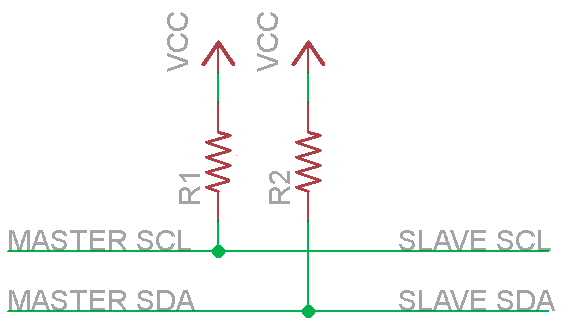
\includegraphics[width=0.3\textwidth]{i2cElectrical.png}
\end{figure}
\begin{itemize}
    \item both lines are connected to positive supply voltage through pull-up resistor
    \item bus driver are open-drain or open-collector
    \item no. of device also depends on the bus capacitance limit of 400pF
\end{itemize}

\section{Data Transfer and Frame Format}

\subsection{Transferring Bits}
\begin{figure}[H]
    \centering
    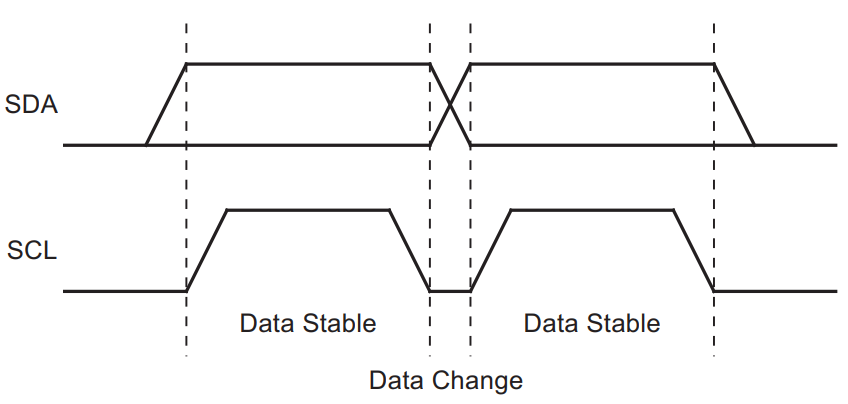
\includegraphics[width=0.5\textwidth]{i2cTransferBits.png}
\end{figure}
\begin{itemize}
    \item Each data bit transferred is done by a pulse on clock line.
    \item Level of data line must be stable when the clock line is high.
\end{itemize}

\subsection{START and STOP Conditions}
\begin{figure}[H]
    \centering
    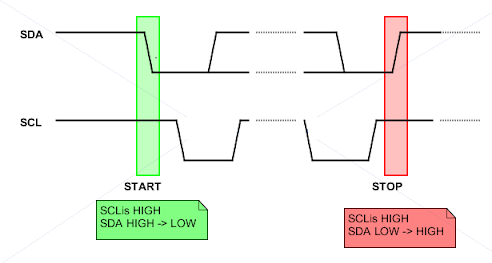
\includegraphics[width=0.7\textwidth]{i2cSTARTSTOP.png}
\end{figure}
\begin{itemize}
	\item Both \iicFormat{START} and \iicFormat{STOP} conditions are done by changing \pinFormat{SDA} line when \pinFormat{SCL} is kept high.
	\item Master initiates transmission by issuing a \iicFormat{START} condition.
	\item Master terminates transmission by issuing a \iicFormat{STOP} condition.
	\item Between \iicFormat{START} and \iicFormat{STOP}, bus is busy and no other master should try to control bus.
	\item The same master however can issue \iicFormat{REPEATED START}(same as \iicFormat{START}) to initiate a new transfer.
\end{itemize}

\subsection{Address Packet format}
    \begin{figure}[H]
        \begin{center}
            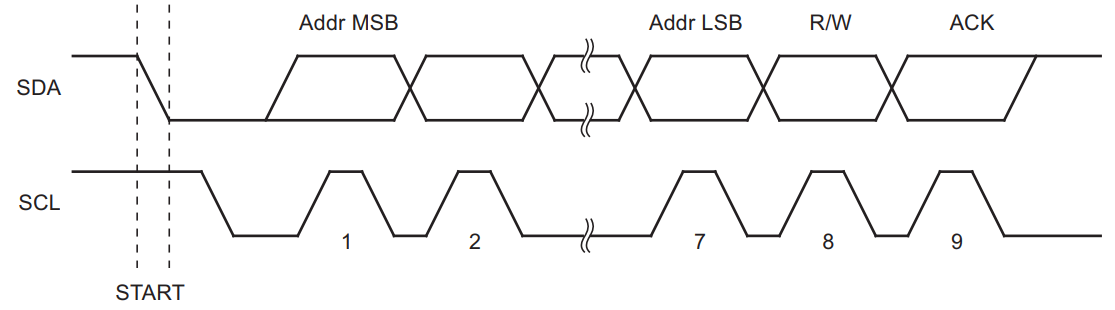
\includegraphics[width=0.8\textwidth]{i2cAddressPacketFormat}
        \end{center}
    \end{figure}
\begin{itemize}
	\item Addresses packets(\iicFormat{SLA}) are 9-bit long.
	\begin{itemize}
		\item 7 address bits with MSB transmitted first
		\item one READ(1)/WRITE(0) control bit indicating the transmitter or receiver mode respectively
		\item one acknowledge bit by the Slave	
	\end{itemize}	
	\item Would take 8 clock cycles by the master to send 7 address bits and one READ/WRITE control bit. \iicFormat{SLA+R} or \iicFormat{SLA+W}.
	\item On the 9th clock cycle, Master will leave out the control of \pinFormat{SDA} line (making it high due to pull-up resistor) but clocks out the 9th clock on the \pinFormat{SCL} line.
	\item On the 9th clock cycle, Slave recognizes that it is being addressed by pulling \pinFormat{SDA} line low making the \iicFormat{ACK}.
	\item If the Slave couldn’t for some reason respond, the \pinFormat{SDA} line remains high in the 9th clock cycle making the \iicFormat{NACK}.
\end{itemize}

\subsection{Data Packet format}
\begin{itemize}
	\item Data packetsare 9-bit long.
	\begin{itemize}
		\item one data byte - 8 bits with MSB first.
		\item one acknowledge bit by the master or slave depending the mode.
	\end{itemize}
	\item The transmitter(either the master or slave) send 8-bit data in 8 clock cycles.
	\begin{figure}[H]
		\begin{center}
			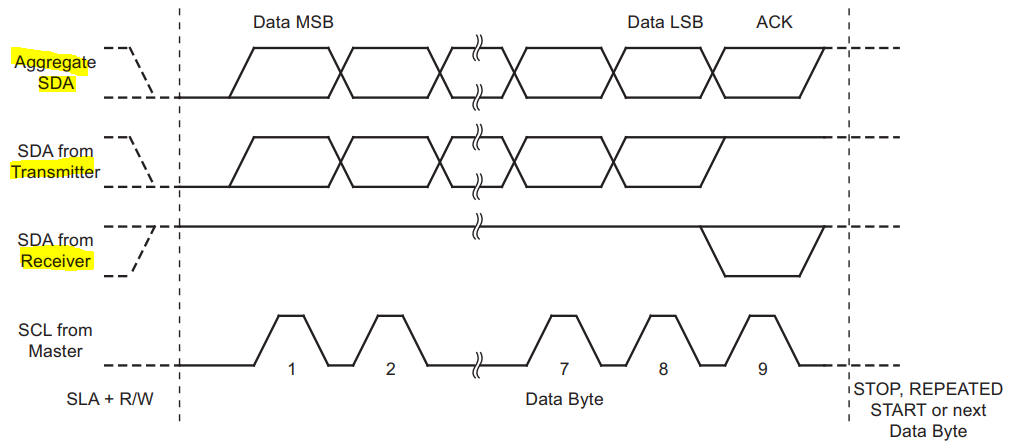
\includegraphics[width=0.8\textwidth]{i2cDataFrame}
		\end{center}
	\end{figure}
	\item On the 9th clock cycle, the transmitter will leave out the control of \pinFormat{SDA} line (making it high due to pull-up resistor).
	\item During the 9th clock cycle, the receiver pulls down the \pinFormat{SDA} line low to acknowledge the reception. – \iicFormat{ACK} is signaled by receiver.
	\item If the receiver doesn’t pull down the \pinFormat{SDA} line for some reason, then the \pinFormat{SDA} line remains high. – \iicFormat{NACK} is signaled by receiver.
	\item When the receiver received the last byte or can’t receive more byte, it should inform the transmitter by sending a \iicFormat{NACK}.
\end{itemize}
\subsection{Overall Operation}
\subsubsection*{Write Operation}
\begin{tikztimingtable}[%
    timing/dslope=0.1,
    timing/.style={x=5ex,y=2ex},
    x=5ex,
    timing/rowdist=3ex,
    timing/name/.style={font=\sffamily\scriptsize}
    ]
    \busref{SDA} & h l l l D{A6} D{A5} [dotted] D{}; D{A0} D{R}
    D{$\overline{ACK}$}
    D{D7} D{D6} [dotted] D{}; D{D0}
    D{$\overline{ACK}$}
    D{D7} D{D6} [dotted] D{}; D{D0}
    D{NACK}
    L l H
     \\
    \busref{SCL} & 0.75H l l l 15{h l} h l l l H 0.5h\\
\end{tikztimingtable}
\subsubsection*{Read Operation}
\begin{tikztimingtable}[%
    timing/dslope=0.1,
    timing/.style={x=5ex,y=2ex},
    x=5ex,
    timing/rowdist=3ex,
    timing/name/.style={font=\sffamily\scriptsize}
    ]
    \busref{SDA} & h l l l D{A6} D{A5} [dotted] D{}; D{A0} D{R}
    D{$\overline{ACK}$}
    D{D7} D{D6} [dotted] D{}; D{D0}
    D{$\overline{ACK}$}
    D{D7} D{D6} [dotted] D{}; D{D0}
    D{NACK}
    L l H
     \\
    \busref{SCL} & 0.75H l l l 15{h l} h l l l H 0.5h\\
\end{tikztimingtable}

\newpage

\section{TWI Module}
\subsection{Block Diagram}
\begin{figure}[H]
    \centering
    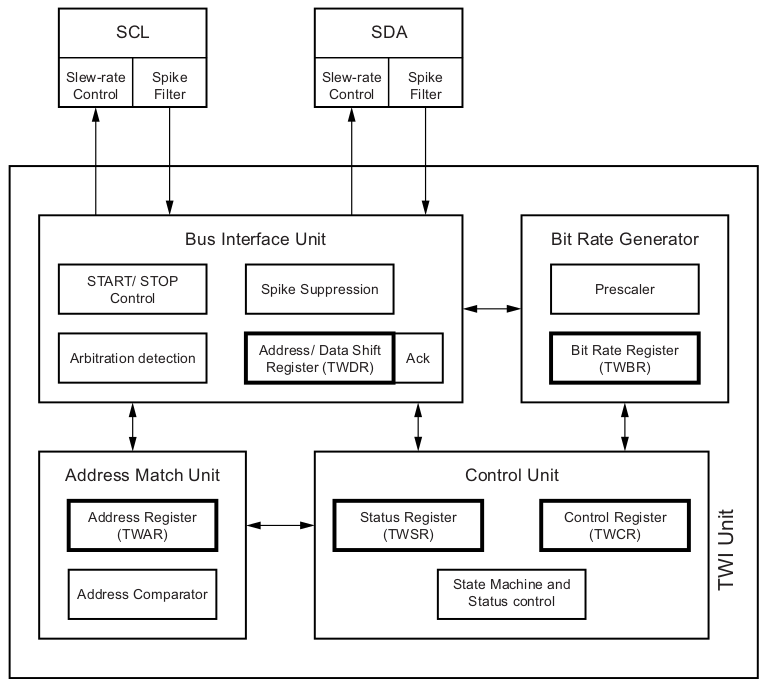
\includegraphics[width=1\textwidth]{TWIModuleOVerview.png}
\end{figure}
\subsection{Bit Rate Generation Unit}
\begin{itemize}
    \item controls \pinFormat{SCL} line when in Master mode
    \item \bitFormat{TWBR} (TWI Bit Rate Generator) and Prescalar Bits in TWI status register \regFormat{TWSR} control \pinFormat{SCL}
    \item The \pinFormat{SCL} frequency can be
\end{itemize}
\begin{center}
    $SCL frequency = \frac{CPU Clock Frequency}{16 + 2 * TWBR * Prescalar Value}$
\end{center}
\textbf{Note: } Slave’s clock frequency must be atleast 16 times higher than SCL frequency.

\subsection{Bus Interface Unit}
\begin{itemize}
    \item contains Data and adress Shift register - \regFormat{TWDR} register - address or data transmitted or received
    \item \iicFormat{START/STOP} Controller - Generates and detects \iicFormat{START}, \iicFormat{STOP} and \iicFormat{REPEATED START}
    \item Register Containing the \iicFormat{(N)ACK} to be transmitted or received
    \item Arbitration detection hardware.
\end{itemize}

\subsection{Address Match Unit}
\begin{itemize}
    \item Received address bytes matches the seven-bit address in \regFormat{TWAR} (TWI Address register).
    \item address match results in informing the control unit
\end{itemize}

\subsection{Control Unit}
\begin{itemize}
    \item Monitors TWI bus and generates responses based on TWI control register (\regFormat{TWCR}).
    \item When a en even requires attention:
    \begin{itemize}
        \item \bitFormat{TWINT} (TWI Interrupt flag ) is set 
        \item \regFormat{TWSR} (TWI Status Register) is updated with status code identifying the event.
        \item when the \bitFormat{TWINT} is set, the \pinFormat{SCL} line is held low.
    \end{itemize}
    \item \bitFormat{TWINT} flag is set If
    \begin{itemize}
        \item TWI has transmitted a \iicFormat{START/REPEATED START} condition
        \item TWI has transmitted \iicFormat{SLA+R/W}
        \item TWI has transmitted an address byte
        \item TWI has lost arbitration
        \item TWI has been addressed by own slave address or general call
        \item TWI has received a data bye
        \item \iicFormat{STOP} or \iicFormat{REPEATED START} has been received
        \item bus error occurred due to illegal \iicFormat{START} or \iicFormat{STOP}
    \end{itemize}
\end{itemize}

\section{TWI Usage}
\begin{itemize}
    \item TWI is interrupt based and so \bitFormat{TWIE} bit in \regFormat{TWCR} register should be enabled; If the \bitFormat{TWIE} is diabled, then the \bitFormat{TWINT} flag must be polled.
    \item When the \bitFormat{TWINT} flag is asserted, TWI has finised operation and awaits for application response and \regFormat{TWSR} register describes the current status of TWI bus.
    \item Then, application should respond by manipulating the \regFormat{TWCR} and \regFormat{TWDR} register.
\end{itemize}

\subsection{An Example - Master transmits single data byte to slave}
\begin{figure}[H]
    \centering
    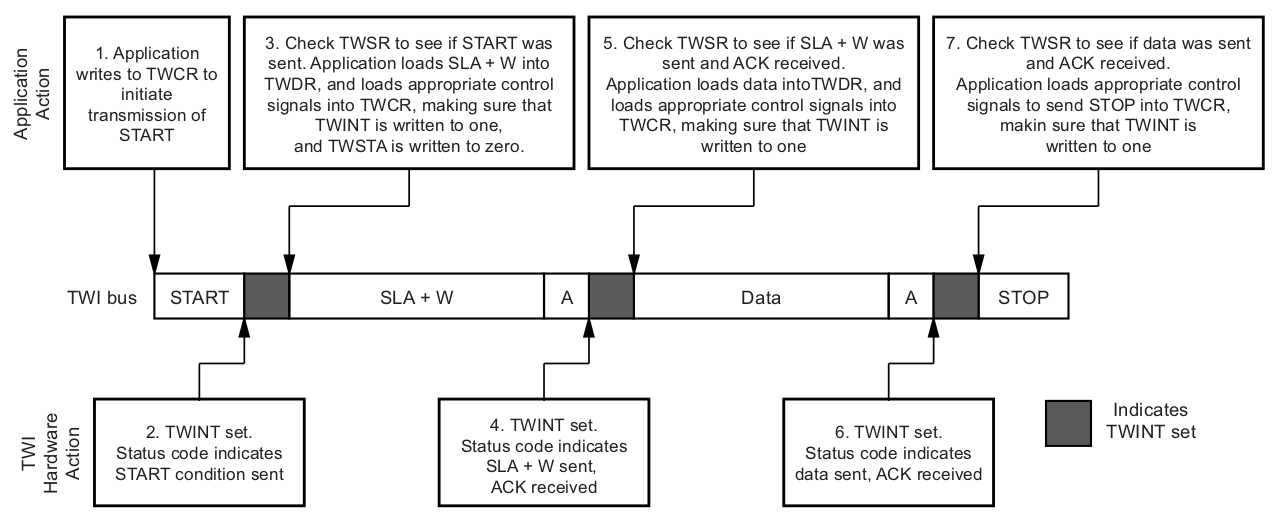
\includegraphics[width=1\textwidth]{TWIExample.png}
\end{figure}
\begin{enumerate}
    \item Transmission is started by writing specific value into \regFormat{TWCR} register to transmit the \iicFormat{START} condition. The \bitFormat{TWINT} flag is cleared by writing Loging HIGH which initiate the transmission of \iicFormat{START} condition.
    \item When the \iicFormat{START} condition has been transmitted, the TWINT flag in TWCR is set, and \regFormat{TWSR} is updated with a status code indicating that the \iicFormat{START} condition has successfully been sent.
    \item The application should now respond by examining the \regFormat{TWSR} register value. If status code is as expected, the application loads \iicFormat{SLA+W} into \regFormat{TWDR} and a specific value is written into \regFormat{TWCR} register to transmit the \iicFormat{SLA+W} present in \regFormat{TWDR}. The \bitFormat{TWINT} flag is cleared by writing logic HIGH which initiates the transmission of address packet.
    \item When the address packet has been transmitted, the \bitFormat{TWINT} flag in \regFormat{TWCR} is set, and \regFormat{TWSR} is updated with a status code indicating that the address packet has successfully been sent. The status code will also reflect whether a slave acknowledged the packet or not.
    \item The application should now respond by examining the \regFormat{TWSR} register value and \iicFormat{ACK} bit is as expected. If status code is as expected, the application loads Data packet into \regFormat{TWDR} and a specific value is written into \regFormat{TWCR} register to transmit the Data packet present in \regFormat{TWDR}. The \bitFormat{TWINT} flag is cleared by writing logic HIGH which initiates the transmission of data packet.
    \item When the data packet has been transmitted, the \bitFormat{TWINT} flag in \regFormat{TWCR} is set, and \regFormat{TWSR} is updated with a status code indicating that the data packet has successfully been sent. The status code will also reflect whether a slave acknowledged the packet or not.
    \item The application should now respond by examining the \regFormat{TWSR} register value and \iicFormat{ACK} bit is as expected. If status code is as expected, the application loads a specific value is written into \regFormat{TWCR} register to transmit the \iicFormat{STOP} Condition. The \bitFormat{TWINT} flag is cleared by writing logic HIGH which initiates the transmission of STOP condition.
\end{enumerate}

\section{Transmission Modes}
\quad There are four major Modes
\begin{enumerate}[label=(\roman*)]
    \item Master Transmitter (MT)
    \item Master Receiver (MR)
    \item Slave Transmitter (ST)
    \item Slave Receiver (SR)
\end{enumerate}
\begin{table}[H]
    \begin{center}
        \begin{tabular}{c|c}
            \textbf{Status Code} & \textbf{Meaning}\\
            \hline
            S & \iicFormat{START} Condition\\
            Rs & \iicFormat{REPEATED START} Condition\\
            R & Read bit (high level on \pinFormat{SDA})\\
            W & Write bit (low level on \pinFormat{SDA})\\
            A & Acknowledge bit (low level on \pinFormat{SDA})\\
            $\overline{A}$ & Not Acknowledge bit (high level on \pinFormat{SDA})\\
            DATA & 8-bit data\\
            P & \iicFormat{STOP} Condition\\
            SLA & Slave Address\\
        \end{tabular}
    \end{center}
\end{table}


\subsection{Master Transmitter Mode (MT)}
\begin{itemize}
    \item Many number of data bytes are transmitted to Slave receiver.
    \item For Master, \iicFormat{START} Condition is transmitted
    \item \iicFormat{START} condition is sent by:
    \begin{itemize}
        \item \bitFormat{TWEN} bit is set to enable TWI.
        \item \bitFormat{TWSTA} bit is set to transmit \iicFormat{START} condition.
        \item \bitFormat{TWINT} flag is written 1 to clear to send start bit.
        \item After Tranmitting \iicFormat{START} condition, \bitFormat{TWINT} flag is set by hardware and status code in \regFormat{TWSR} register should be \statusCode{0x08} - indicating successfull transmission of \iicFormat{START} condition.
    \end{itemize}
    \item  To enter into Master Transmitter Mode and transmit the address:
    \begin{itemize}
        \item Write \iicFormat{SLA+W} into \regFormat{TWDR} register.
        \item \bitFormat{TWINT} flag is written 1 to clear to transmit Address and read/write status.
        \item After transmitting \iicFormat{SLA+W}, an acknowledgment bit will be received, the \bitFormat{TWINT} flag is set by hardware and status code in \regFormat{TWSR} register will be \statusCode{0x18} (indicating \iicFormat{SLA+W} has been transmitted and \iicFormat{ACK} has been received ), \statusCode{0x20} (indicating \iicFormat{SLA+W} has been transmitted and \iicFormat{NACK} has been received ), \statusCode{0x38} (Arbitration lose in sending \iicFormat{SLA+W}).
    \end{itemize}
    \item Data packet is transmitted by:
    \begin{itemize}
        \item Write \iicFormat{DATA} packet into \regFormat{TWDR} register.
        \item \bitFormat{TWINT} flag is written 1 to clear to transmit Address and read/write status.
        \item After transmitting \iicFormat{DATA} packet, an acknowledgment bit will be received, the \bitFormat{TWINT} flag is set by hardware and status code in \regFormat{TWSR} register will be \statusCode{0x28} (indicating  \iicFormat{DATA} packet has been transmitted and \iicFormat{ACK} has been received ), \statusCode{0x30} (indicating  \iicFormat{DATA} packet has been transmitted and \iicFormat{NACK} has been received )
    \end{itemize}
    \begin{itemize}
        \item To send further data, the above process is repeated by sending \iicFormat{REPEATED START}.
        \item To stop the transmission, the \iicFormat{STOP} condition is sent.
    \end{itemize}
    \item \iicFormat{STOP} condition is sent by:
    \begin{itemize}
        \item \bitFormat{TWSTO} bit is set to transmit \iicFormat{STOP} condition.
        \item \bitFormat{TWINT} flag is written 1 to clear to send stop bit.
    \end{itemize}
    \item \iicFormat{REPEATED START} condition is sent by:
    \begin{itemize}
        \item \bitFormat{TWSTA} bit is set to transmit \iicFormat{REPEATED START} condition.
        \item \bitFormat{TWINT} flag is written 1 to clear to send repated start bit.
        \item After Tranmitting \iicFormat{REPEATED START} condition, \bitFormat{TWINT} flag is set by hardware and status code in \regFormat{TWSR} register should be \statusCode{0x10} - indicating successfull transmission of \iicFormat{REPEATED START} condition.
    \end{itemize}
\end{itemize}

\subsection{Master Receiver Mode (MR)}
\begin{itemize}
    \item Many number of data bytes can be received from Slave transmitter.
    \item For Master, \iicFormat{START} Condition is transmitted
    \item \iicFormat{START} condition is sent by:
    \begin{itemize}
        \item \bitFormat{TWEN} bit is set to enable TWI.
        \item \bitFormat{TWSTA} bit is set to transmit \iicFormat{START} condition.
        \item \bitFormat{TWINT} flag is written 1 to clear to send start bit.
        \item After Tranmitting \iicFormat{START} condition, \bitFormat{TWINT} flag is set by hardware and status code in \regFormat{TWSR} register should be \statusCode{0x08} - indicating successfull transmission of \iicFormat{START} condition.
    \end{itemize}
    \item  To enter into Master Receiver Mode and transmit the address:
    \begin{itemize}
        \item Write \iicFormat{SLA+R} into \regFormat{TWDR} register.
        \item \bitFormat{TWINT} flag is written 1 to clear to transmit Address and read/write status.
        \item After transmitting \iicFormat{SLA+R}, an acknowledgment bit will be received, the \bitFormat{TWINT} flag is set by hardware and status code in \regFormat{TWSR} register will be \statusCode{0x40} (indicating \iicFormat{SLA+R} has been transmitted and \iicFormat{ACK} has been received ), \statusCode{0x48} (indicating \iicFormat{SLA+R} has been transmitted and \iicFormat{NACK} has been received ), \statusCode{0x38} (Arbitration lose in sending \iicFormat{SLA+R}).
    \end{itemize}
    \item Data packet is received by:
    \begin{itemize}
        \item Reading the \iicFormat{DATA} packet from \regFormat{TWDR} register if \bitFormat{TWINT} flag is logic HIGH.
        \item \bitFormat{TWINT} flag is written 1 to clear.
        \item After receiving \iicFormat{DATA} packet, an acknowledgment bit will be returned, the \bitFormat{TWINT} flag is set by hardware and status code in \regFormat{TWSR} register will be \statusCode{0x58} (indicating  \iicFormat{DATA} packet has been recieved and \iicFormat{ACK} has been returned ), \statusCode{0x50} (indicating  \iicFormat{DATA} packet has been recieved and \iicFormat{NACK} has been returened )
    \end{itemize}
    \begin{itemize}
        \item To receive further data, the above process is repeated by sending \iicFormat{REPEATED START}.
        \item To stop the reception, the \iicFormat{STOP} condition is sent.
    \end{itemize}
    \item \iicFormat{STOP} condition is sent by:
    \begin{itemize}
        \item \bitFormat{TWSTO} bit is set to transmit \iicFormat{STOP} condition.
        \item \bitFormat{TWINT} flag is written 1 to clear to send stop bit.
    \end{itemize}
    \item \iicFormat{REPEATED START} condition is sent by:
    \begin{itemize}
        \item \bitFormat{TWSTA} bit is set to transmit \iicFormat{REPEATED START} condition.
        \item \bitFormat{TWINT} flag is written 1 to clear to send repated start bit.
        \item After Tranmitting \iicFormat{REPEATED START} condition, \bitFormat{TWINT} flag is set by hardware and status code in \regFormat{TWSR} register should be \statusCode{0x10} - indicating successfull transmission of \iicFormat{REPEATED START} condition.
    \end{itemize}
\end{itemize}

\subsection{Slave Receiver Mode (SR)}
\begin{itemize}
    \item Many number of data bytes are received from Master transmitter.
    \item To initiate the Slave Mode:
    \begin{itemize}
        \item \bitFormat{TWA[5:0]} bits from \regFormat{TWAR} regFormat is loaded with our slave address.
        \item \bitFormat{TWSTA} and \bitFormat{TWSTO} are set to 0
        \item \bitFormat{TWEN} bit is set to enable the TWI.
    \end{itemize}
    \item TWI waits until it is addressed by its own slave address followed by data direction bit.
    \item After receiving own Slave address and Write bit, the \bitFormat{TWINT} flag is set and valid status code is available in \regFormat{TWSR} register.
    \item If the status code is \statusCode{0x60} (Own \iicFormat{SLA+W} has been recieved and \iicFormat{ACK} has been returned)
    \item Now, data can be read by wiring Logic HIGH on \bitFormat{TWINT} flag to clear and read from \regFormat{TWDR} register.
    \item \bitFormat{TWEA} bit is set to acknowledge and recieve further data or \bitFormat{TWEA} bit is cleared and last byte is received.
    \item Now, \bitFormat{TWINT} flag is set and status code is avalaible in \regFormat{TWSR}.
    \item If status code is \statusCode{0x80} (Previously addressed with own \iicFormat{SLA+W} and data has been received and \iicFormat{ACK} has been returned) - to receive further data.
    \item If status code is \statusCode{0x88} (Previously addressed with own \iicFormat{SLA+W} and data has been received and \iicFormat{NACK} has been returned) - last data is recieved.
    \item If status code is \statusCode{0xA0} -  A \iicFormat{STOP} condition is recieved.
    has been received
\end{itemize}

\subsection{Slave Transmitter Mode (ST)}
\begin{itemize}
    \item Many number of data bytes are transmitted to Master recive.
    \item To initiate the Slave Mode:
    \begin{itemize}
        \item \bitFormat{TWA[5:0]} bits from \regFormat{TWAR} regFormat is loaded with our slave address.
        \item \bitFormat{TWSTA} and \bitFormat{TWSTO} are set to 0
        \item \bitFormat{TWEN} bit is set to enable the TWI.
    \end{itemize}
    \item TWI waits until it is addressed by its own slave address followed by data direction bit.
    \item After receiving own Slave address and Read bit, the \bitFormat{TWINT} flag is set and valid status code is available in \regFormat{TWSR} register.
    \item If the status code is \statusCode{0xA8} (Own \iicFormat{SLA+R} has been recieved and \iicFormat{ACK} has been returned)
    \item Now, data to be sent is set on the \regFormat{TWDR} register.
    \item \bitFormat{TWINT} flag is written 1 to clear to transmit the data.
    \item Now, \bitFormat{TWINT} flag is set and status code is avalaible in \regFormat{TWSR}.
    \item If status code is \statusCode{0xB8} -(Data byte in \regFormat{TWDR} has been transmitted and \iicFormat{ACK} has been received) - can send further data.
    \item If status code is \statusCode{0xC8} -(Data byte in \regFormat{TWDR} has been transmitted and \iicFormat{NACK} has been received) - last byte send and dont' send further.
\end{itemize}

\section{Register Desciption}
\subsubsection*{TWBR – TWI Bit Rate Register}
\vspace*{0.5cm}
\begin{bytefield}[bitformatting={\large\bfseries},
    endianness=big,bitwidth=0.125\linewidth]{8}
    \bitheader[lsb=0]{0-7} \\
    \bitbox{8}{\small TWBR[7:0]}\\
\end{bytefield}

\quad The bit rate is found by,
\begin{center}
    $SCL frequency = \frac{CPU Clock Frequency}{16 + 2 * TWBR * Prescalar Value}$
\end{center}

\subsubsection*{TWCR – TWI Control Register}
\vspace*{0.5cm}
\begin{bytefield}[bitformatting={\large\bfseries},
    endianness=big,bitwidth=0.125\linewidth]{8}
    \bitheader[lsb=0]{0-7} \\
    \bitbox{1}{\small TWINT}
    \bitbox{1}{\small TWEA}
    \bitbox{1}{\small TWSTA}
    \bitbox{1}{\small TWSTO}
    \bitbox{1}{\small TWWC}
    \bitbox{1}{\small TWEN}
    \bitbox{1}{\small -}
    \bitbox{1}{\small TWIE}\\
\end{bytefield}
\begin{itemize}
    \item \bitFormat{TWINT} - TWI Interrupt Flag - Set by hardware when TWI has finished its current job and expects applicaion software reponse. This Flag should be cleared by software by writing login HIGH to start the operation of TWI.
    \item \bitFormat{TWEA} - TWI Enable Acknowledge Bit - Controls the genration of acknowledge pulse.
    \item \bitFormat{TWSTA} - TWI \iicFormat{START} condition - to generate \iicFormat{START} or \iicFormat{REPEATED START}.
    \item \bitFormat{TWSTO} - TWI \iicFormat{STOP} condition - to Generate \iicFormat{STOP} condition.
    \item \bitFormat{TWEN} - TWI Enable Bit - To enabled and active TWI interface - takes control over \pinFormat{SDA} and \pinFormat{SCL} pins, enables slew-rate limiter and spike filter.
    \item \bitFormat{TWIE} - TWI Interrupt ENable - to enable interrupt when TWI flag is high.
\end{itemize}

\subsubsection*{TWSR – TWI Status Register}
\vspace*{0.5cm}
\begin{bytefield}[bitformatting={\large\bfseries},
    endianness=big,bitwidth=0.125\linewidth]{8}
    \bitheader[lsb=0]{0-7} \\
    \bitbox{5}{\small TWS[7:3]}
    \bitbox{1}{\small -}
    \bitbox{1}{\small TWPS1}
    \bitbox{1}{\small TWPS2}\\
\end{bytefield}

\begin{itemize}
    \item \bitFormat{TWS[7:3]} - TWI Status - reflects the status of TWI logic and 2-wire status bus.
\end{itemize}

\begin{table}[H]
    \begin{center}
        \begin{tabular}{c|c}
            \bitFormat{TWPS[1:0]} \textbf{- TWI Bit rate Prescalar} & \textbf{Prescaler Value}\\
            \hline
            00 & 1\\
            01 & 4\\
            10 & 16\\
            11 & 64\\
        \end{tabular}
    \end{center}
\end{table}

\subsubsection*{TWDR – TWI Data Register}
\vspace*{0.5cm}
\begin{bytefield}[bitformatting={\large\bfseries},
    endianness=big,bitwidth=0.125\linewidth]{8}
    \bitheader[lsb=0]{0-7} \\
    \bitbox{8}{\small TWD[7:0]}\\
\end{bytefield}

\subsubsection*{TWAR – TWI (Slave) Address Register}
\vspace*{0.5cm}
\begin{bytefield}[bitformatting={\large\bfseries},
    endianness=big,bitwidth=0.125\linewidth]{8}
    \bitheader[lsb=0]{0-7} \\
    \bitbox{7}{\small TWA[6:0]}
    \bitbox{1}{\small TWGCE}\\
\end{bytefield}

\begin{itemize}
    \item \bitFormat{TWA[6:0]} - TWI Slave adress Register - contain seven bit slave address.
    \item \bitFormat{TWGCE} - TWI General Call Recogniction Bit - enables the recognition of general call.
\end{itemize}

\section{Configuring the I2c}
\subsection{Master Transmitter and Receiver}

\quad The code can be seen below:

\begin{minted}[breaklines, bgcolor=lightgray]{c}
uint8_t status = 0;
void I2C_Master_Init()
{
	// Intialize the I2C clock frequency to 100kHz
	// let the prescalr be 1
	// f_i2c =  F_CPU / (16 + (2*xTWBR*Prescaler)) = 32
	// setting the TWBR register.
	TWBR = 32;

	// writing 1 to prscalre
	// setting the TWPS bits in TWSR to 00
	TWSR &= ~(1<<TWPS0);
	TWSR &= ~(1<<TWPS1);
}
uint8_t I2C_Master_Status()
{
	// Status value are available from TWSR[7:3]
	return TWSR & 0XF8;
}
uint8_t I2C_Master_START()
{
	// Enabling the TWI interface
	TWCR |= (1<<TWEN);
	// sending START condition
	TWCR |= (1<<TWSTA);
	// Do the transaction
	TWCR |= (1<<TWINT);
	// Checking if START condition is sent correctly
	while((TWCR & (1<<TWINT )) == 0x00);
	status = I2C_Master_Status();
	// checking status if START condition is sent correctily
	if(status == 0x08)
	{
		// no error occured
		return 0;
	}
	else
	{
		// error occured
		return 0;
	}
}
uint8_t I2C_Master_STOP()
{
	// Removing Start condition on bit
	TWCR &= ~(1<<TWSTA);
	// sending STOP condition
	TWCR |= (1<<TWSTO);
	
	// Do the transaction
	TWCR |= (1<<TWINT);

	// disaabling stop and interface
	
	
	TWCR &= ~(1<<TWSTO);
	TWCR &= ~(1<<TWEN);

	return 0;
}
uint8_t I2C_Master_Mode(uint8_t slave_address, uint8_t transmiter0_receiver1)
{
	// Entering MASTER mode
	// Writing SLA+W into TWDR for transmiiter and SLA+R for receiver
	// slave address must be MSB first
	// slave address is left shifted by 1 in order to accompany the R/W bit
	TWDR = (slave_address<<1) | transmiter0_receiver1;
	// Do the transaction
	TWCR |= (1<<TWINT);
	while((TWCR & (1<<TWINT )) == 0x00);
	status = I2C_Master_Status();
	// For transmitter the staus would have to be 0x18 and for receiver 0x40
	uint8_t status_val_checker = (transmiter0_receiver1==0) ? 0x18 : 0x40;
	if(status == status_val_checker)
	{
		// no error occured
		return 0;
	}
	else
	{
		// error occured
		return 0;
	}
}
uint8_t I2C_Master_DataTransmitByte(uint8_t data_)
{
	// Data packet is transmitted
	// Writing data intor TWDR
	TWDR = data_;
	// Do the transaction
	TWCR |= (1<<TWINT);
	while((TWCR & (1<<TWINT )) == 0x00);
	status = I2C_Master_Status();
	if(status == 0x28)
	{
		// ACK received and still data can be sent
		return 0;
	}
	else if(status == 0x30)
	{
		// NACK received and this is the last data so stop
		return 1;
	}
	else
	{
		// error occured
		return 2;
	}
}
void I2C_Master_DataTransmitString(uint8_t *cdata)
{
	while(*cdata != '\0')
	{
		status = I2C_Master_DataTransmitByte(*cdata++) ;
		if(status == 0)
		{
			// ACK received and still data can be sent
			// continue
		}
		else if(status == 1)
		{
			// NACK received and this is the last data so stop
			return;
		}
		else
		{
			// error occured
			return;
		}
	}
}

uint8_t I2C_Master_DataReceiveByte()
{
	uint8_t value_ = 0;

	// Data packet is recieved
	TWCR |= (1<<TWINT);
	// Do the transaction
	while((TWCR & (1<<TWINT )) == 0x00)
	{
		value_ = TWDR;
	}
	
	 	
	status = I2C_Master_Status();
	if(status == 0x58)
	{
		// no error occured
		return value_;
	}
	else
	{
		// error occured
		return 1;
	}
}
void I2C_Master_DataReceiveString(uint8_t *recData,uint8_t NUMBYTE)
{
	uint8_t i=0;
	recData[NUMBYTE] = '\0';
	while(i < NUMBYTE)
	{
		// Enabling the Acknowledment bit for replying positive ACK
		TWCR |= (1<<TWEA);
		if(i==(NUMBYTE-1))
		{
			// disbale the Acknowledment bit for replying Negatice ACK for last byte
			TWCR &= ~(1<<TWEA);
		}
		status = I2C_Master_DataReceiveByte();
		if(status==0xFF)
			return;
		else		
			recData[i] = status;
		i++;
	}
}
\end{minted}

\newpage
\subsection{Slave Transmitter and Receiver}

\quad The code can be seen below:

\begin{minted}[breaklines, bgcolor=lightgray]{c}
uint8_t status = 0;
void I2C_SlaveInit(uint8_t my_address)
{
	// slave address  and last LSB 0 is for general call
	TWAR = (my_address<<1) & 0xFE;
	// Enabling the TWI interface.
	TWCR |= (1<<TWEN);
	// Disabling Start and Stop conditon bits
	TWCR &= ~(1<<TWSTA);
	TWCR &= ~(1<<TWSTO);

}
uint8_t I2C_Status()
{
	// Status value are available from TWSR[7:3]
	return TWSR & 0XF8;
}

uint8_t I2C_SlaveMode( uint8_t transmiter0_receiver1)
{
	// Acknowldege the address
	TWCR |= (1<<TWEA);
	// Watiting for the Master to call this slave
	while((TWCR & (1<<TWINT )) == 0x00);
	status = I2C_Status();
	// For transmitter the staus would have to be 0xA8 and for receiver 0x60
	uint8_t status_val_checker = (transmiter0_receiver1==0) ? 0xA8 : 0x60;
	if(status == status_val_checker)
	{
		// Master called this slave
		return 0;
	}
	else
	{
		// error occured
		return 1;
	}
}
uint8_t I2C_Slave_DataTransmitByte(uint8_t data_)
{
	// Data packet is transmitted
	// Writing data intor TWDR
	TWDR = data_;
	// Do the transaction
	TWCR |= (1<<TWINT);
	while((TWCR & (1<<TWINT )) == 0x00);

	status = I2C_Status();
	if(status == 0xB8)
	{
		// ACK received and still data can be sent
		return 0;
	}
	else if(status == 0xC8)
	{
		// NACK received and this is the last data so stop
		return 1;
	}
	else
	{
		// error occured
		return 2;
	}
}
void I2C_Slave_DataTransmitString(char *cdata)
{
	uint8_t i = 0;
	while(cdata[i] != '\0')
	{
		status = I2C_Slave_DataTransmitByte(cdata[i]) ;
		i++;
		if(status == 0)
		{
			// ACK received and still data can be sent
			// continue
		}
		else if(status == 1)
		{
			// NACK received and this is the last data so stop
			return;
		}
		else
		{
			// error occured
			return;
		}
	}
}

uint8_t I2C_Slave_DataReceiveByte()
{
	uint8_t value_ = 0;

	// Data packet is recieved
	TWCR |= (1<<TWINT);
	// Do the transaction
	while((TWCR & (1<<TWINT )) == 0x00)
	{
		value_ = TWDR;
	}
	
	status = I2C_Status();
	if(status == 0x80)
	{
		// Data is sent and ACK has been returned
		return value_;
	}
	else if(status == 0x88)
	{
		// Data is sent and NACK has been returned for last byte
		return value_;
	}
	else
	{
		// error occured
		return 0xFF;
	}
}
void I2C_Slave_DataReceiveString(uint8_t *recData,uint8_t NUMBYTE)
{
	uint8_t i=0;
	recData[NUMBYTE] = '\0';
	while(NUMBYTE > 0)
	{
		NUMBYTE = NUMBYTE - 1;
		// Enabling the Acknowledment bit for replying positive ACK
		TWCR |= (1<<TWEA);
		if(NUMBYTE==0)
		{
			// disbale the Acknowledment bit for replying Negatice ACK for last byte
			TWCR &= ~(1<<TWEA);
		}
		status = I2C_Slave_DataReceiveByte();
		if(status==0xFF)
			return;
		else		
			recData[i] = status;
		i++;
	}
}
\end{minted}

\end{document}
